% !TEX TS-program = xelatex
% !TEX encoding = UTF-8 Unicode
% !Mode:: "TeX:UTF-8"

\documentclass{resume}
\usepackage[dvipsnames,svgnames]{xcolor}
\usepackage{zh_CN-Adobefonts_external} % Simplified Chinese Support using external fonts (./fonts/zh_CN-Adobe/)
% \usepackage{NotoSansSC_external}
% \usepackage{NotoSerifCJKsc_external}
% \usepackage{zh_CN-Adobefonts_internal} % Simplified Chinese Support using system fonts
\usepackage{linespacing_fix} % disable extra space before next section
\usepackage{cite}
\usepackage{tabu}
\usepackage{multirow}
\usepackage{progressbar}
\usepackage[most]{tcolorbox}
\newtcbox{\badge}[1][red]{
  on line, 
  arc=2pt,
  colback=#1!50!black,
  colframe=#1!50!black,
  fontupper=\color{white},
  boxrule=1pt, 
  boxsep=0pt,
  left=6pt,
  right=6pt,
  top=2pt,
  bottom=2pt
}

\begin{document}
\pagenumbering{gobble} % suppress displaying page number

\Large{
  \begin{tabu}{ c l r }
    \multirow{5}{1in}{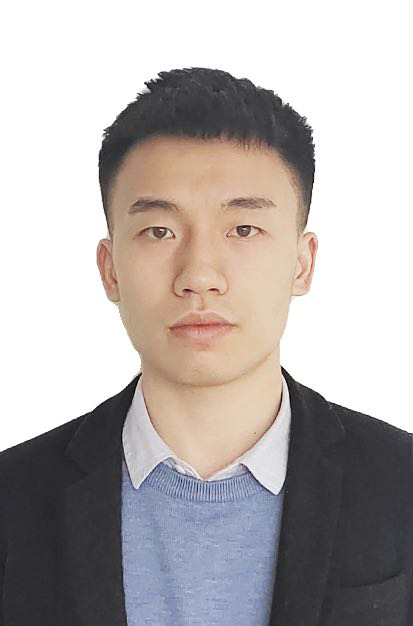
\includegraphics[width=0.80in]{WechatIMG1}} &  & {路由\&交换~}\progressbar[ticksheight=0]{0.6} \\
    & \scshape{林帅} & {Linux~}\progressbar[ticksheight=0]{0.5} \\
    & \email{lsplub@gmail.com} & {Sql~}\progressbar[ticksheight=0]{0.4} \\
    & \phone{(+86) 131-988-98368} & {Golang~\&web~}\progressbar[ticksheight=0]{0.6} \\
    & \github[github.com/triment]{https://github.com/triment} & {数据结构~}\progressbar[ticksheight=0]{0.3}
  \end{tabu}
}
 
\section{\faUsers\ 工作经历}
\datedsubsection{\textbf{四川壹米滴答供应链管理有限公司} }{2020年3月 -- 至今}
\role{运维经理}{IT支持组} ~\badge[TealBlue]{2021年一季度优秀团队} ~\badge[TealBlue]{两次总部内推(运维测试岗)}
\begin{itemize}
  \item 负责转运中心机房弱电设备(防火墙、交换机、AC、AP 等)和桌面维护😄
  \item IT服务数据监控,业务功能需求分析
  \item 编写自动化网络测试工具(flutter-安卓端),excel数据处理工具(golang)
\end{itemize}

\datedsubsection{\textbf{诺可思科技有限公司}}{2018年12月 -- 2020年3月}
\role{信息学教师}{教研部}
~\badge[TealBlue]{成都市创意编程比赛一等奖}
\begin{itemize}
  \item 负责 Python、C++ 青少年课程开发、教材编写,以及相关练习题、信息学试卷制作(\LaTeX 排版)
  \item 定期定时到合作学校授课,带领学员参加青少年创意编程比赛、蓝桥杯编程比赛
\end{itemize}



% Reference Test
%\datedsubsection{\textbf{Paper Title\cite{zaharia2012resilient}}}{May. 2015}
%An xxx optimized for xxx\cite{verma2015large}
%\begin{itemize}
%  \item main contribution
%\end{itemize}

\section{\faCogs\ IT 技能}
% increase linespacing [parsep=0.5ex]
\begin{itemize}[parsep=0.5ex]
  \item 编程语言: golang,javascript(es6),python
  \item 平台工具: Linux, Mac,vscode,docker-compose,华为网络设备调试
  \item 开发: react,golang,flutter,nodejs
\end{itemize}

\section{\faGithub\ 作品(部分)}
% increase linespacing [parsep=0.5ex]
\begin{itemize}[parsep=0.5ex]
  \item eject: https://github.com/triment/eject 一个restful微型后端框架~\badge[Aquamarine]{golang}
  \item react-markdown-editor: https://github.com/Triment/react-markdown-editor 一个支持数学公式的markdown编辑器~\badge[Aquamarine]{react}
\end{itemize}

\section{\faGraduationCap\  教育背景}
\datedsubsection{\textbf{成都信息工程}}{2019 -- 2021}
\textit{专科}\ 计算机应用技术

\section{\faSunO\ 其他介绍}

具有良好的沟通、协作能力,有良好的职业道德和较强的工作责任感。

熟悉\textbf{计算机网络},独立配置过园区网络。熟悉计算机软硬件维护,服务器维护,有编程基础,能编写自动化脚本。
%% Reference
%\newpage
%\bibliographystyle{IEEETran}
%\bibliography{mycite}
\end{document}
